% Aufgabe: Messaufgaben auflisten
% Vorbereitung: Vorbereitungsaufgaben bearbeiten
% Versuchsaufbau: Verwendete Apparatur, Beschreibung Funktionsweise/Nutzen mit Skizze/Foto
\section{Durchführung}
\label{sec:durchführung}

\begin{figure}[H]
	\centering
	\vspace{1.23ex}
	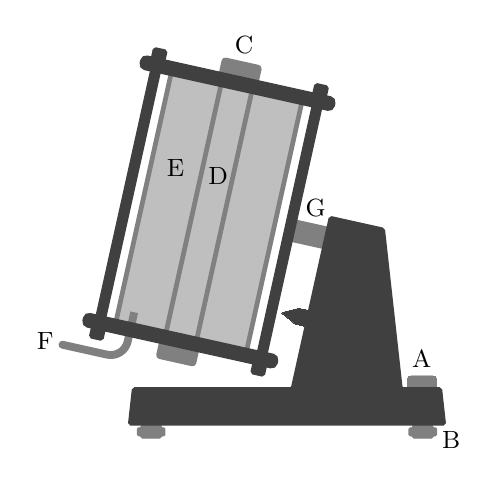
\begin{tikzpicture}
		\tikzstyle{every node} = [font = \small]

% Füße
\draw[draw = gray, fill = gray, rounded corners = 0.15mm]
	(0.15,0) -- ++(0,-0.0475) -- ++(-0.05,0) -- ++(0,-0.1) -- ++(0.05,0) -- ++(0,-0.03) --
	++(0.25,0) -- ++(0,0.03) -- ++(0.05,0) -- ++(0,0.1) -- ++(-0.05,0) -- ++(0,0.0475);
\draw[draw = gray, fill = gray, rounded corners = 0.15mm]
	(3.6,0) -- ++(0,-0.0475) -- ++(-0.05,0) -- ++(0,-0.1) -- ++(0.05,0) -- ++(0,-0.03) --
	++(0.25,0) -- ++(0,0.03) -- ++(0.05,0) -- ++(0,0.1) -- ++(-0.05,0) -- ++(0,0.0475);

% Libelle
\draw[draw = lightgray, fill = lightgray, line width = 0mm, rounded corners = 0mm]
	(3.53,0.599) [rounded corners = 0.75mm] -- ++(0,0.025) -- ++(0.365,0) [rounded corners = 0.75mm] -- ++(0,-0.025);
\fill[white, even odd rule]
	(3.5,0.7) rectangle (4,0.5)
	(3.551,0.7) rectangle (3.874,0.5);
\draw[draw = gray, fill = gray, line width = 0mm, rounded corners = 0.2mm]
	(3.525,0.45) -- ++(0,0.15) -- ++(0.375,0) -- ++(0,-0.15);

% Gefäß
\begin{scope}[rotate = -12.5288077092]
	% Achse
	\draw[draw = gray, fill = gray, line width = 0.4mm]
		(1.5,2.725) -- ++(0.42,0) -- ++(0,0.25) -- ++(-0.42,0);
	% Deckel
	\draw[draw = gray, fill = gray, line width = 0.2mm, rounded corners = 0.4mm]
		(0.15,4.6) -- ++(0,0.2) -- ++(0.5,0) -- ++(0,-0.2);
	\draw[draw = gray, fill = gray, line width = 0.2mm, rounded corners = 0.4mm]
		(0.15,1.1) -- ++(0,-0.2) -- ++(0.5,0) -- ++(0,0.2);
	% Zylinder
	\draw[draw = gray, fill = lightgray, line width = 0mm]
		(-0.45,1.25) -- ++(0,3.2) -- ++(1.7,0) -- ++(0,-3.2) -- cycle;
	\draw[draw = gray, line width = 0.6mm]
		(-0.45,1.25) -- ++(0,3.2);
	\draw[draw = gray, line width = 0.6mm]
		(1.25,1.25) -- ++(0,3.2);
	\draw[draw = gray, line width = 0.6mm]
		(0.2,1.25) -- ++(0,3.2);
	\draw[draw = gray, line width = 0.6mm]
		(0.6,1.25) -- ++(0,3.2);
	% Zufuhr
	\draw[draw = gray, line width = 1mm]
		(-0.25,1.4) -- ++(0,-0.2);
	\draw[draw = gray, line width = 1mm, rounded corners = 2.2mm, line cap = round]
		(-0.25,1.2) -- ++(0,-0.4) -- ++(-0.8,0);
	% Käfig
	\draw[draw = darkgray, fill = darkgray, line width = 0.4mm]
		(1.4,1.25) -- ++(0,3.2) -- ++(0.1,0) -- ++(0,-3.2);
	\draw[draw = darkgray, fill = darkgray, line width = 0.4mm]
		(-0.7,1.25) -- ++(0,3.2) -- ++(0.1,0) -- ++(0,-3.2);
	\draw[draw = darkgray, fill = darkgray, line width = 0.4mm, rounded corners = 0.6mm]
		(-0.85,4.45) -- ++(2.5,0) -- ++(0,0.15) -- ++(-2.5,0) -- cycle;
	\draw[draw = darkgray, fill = darkgray, line width = 0.4mm, rounded corners = 0.6mm]
		(-0.85,1.1) -- ++(2.5,0) -- ++(0,0.15) -- ++(-2.5,0) -- cycle;
	% Schrauben
	\draw[draw = darkgray, fill = darkgray, line width = 0.4mm, rounded corners = 0.2mm]
		(-0.725,4.6) -- ++(0,0.125) -- ++(0.15,0) -- ++(0,-0.125);
	\draw[draw = darkgray, fill = darkgray, line width = 0.4mm, rounded corners = 0.2mm]
		(1.375,4.6) -- ++(0,0.125) -- ++(0.15,0) -- ++(0,-0.125);
	\draw[draw = darkgray, fill = darkgray, line width = 0.4mm, rounded corners = 0.2mm]
		(-0.725,1.1) -- ++(0,-0.125) -- ++(0.15,0) -- ++(0,0.125);
	\draw[draw = darkgray, fill = darkgray, line width = 0.4mm, rounded corners = 0.2mm]
		(1.375,1.1) -- ++(0,-0.125) -- ++(0.15,0) -- ++(0,0.125);
	% Raste
	\draw[draw = darkgray, fill = darkgray, line width = 0mm, rounded corners = 0.1mm]
		(1.575,1.8) -- ++(0.2,-0.1) -- ++(0.3,-0.01) -- ++(0,0.22) -- ++(-0.3,-0.01) -- cycle;	
\end{scope}

% Stativ
\draw[draw = darkgray, fill = darkgray, line width = 0.4mm, rounded corners = 0.2mm]
	(0,0) -- (4,0) -- (3.95,0.45) -- (3.45,0.45) -- (3.225,2.475) --
	(2.55,2.625) -- (2.0666666666666667,0.45) -- (0.05,0.45) -- cycle;

% Kennung
\node at (1.455,4.81) {C};
\node at (1.125,3.15) {D};
\node at (0.585,3.25) {E};
\node at (-1.07,1.05) {F};
\node at (2.364,2.75) {G};
\node at (3.7125,0.825) {A};
\node at (4.085,-0.2) {B};

	\end{tikzpicture}
	\vspace{1.23ex}
	\caption{Schematische Darstellung der Messapparatur.}
	\label{fig:apparat}
\end{figure}

Zunächst werden zwei verschieden große Glaskugeln gewogen und mithilfe einer genormten Bügelmessschraube vermessen.
Anschließend wird an der Libelle \small (A) \normalsize überprüft, ob die Apparatur horizontal eben steht.
Gegebenenfalls kann durch Verstellen der Stützen \small (B) \normalsize nachjustiert werden. Über die beidseitigen
Schraubverschlüsse \small (C) \normalsize wird das Fallrohr \small (D) \normalsize des
Höppler\hspace{0.15ex}-\hspace{-0.15ex}Viskosimeters mit bidestilliertem Wasser gefüllt. Umgeben ist dieses von einem
Wasserbad \small(E)\normalsize, welches über die Anschlüsse \small (F) \normalsize durch ein Thermostat gespeist wird.
So ist für eine stetige Durchmischung sowie ein dadurch gleichmäßiges Temperieren der Flüssigkeit im Fallrohr gesorgt.
Die Wassertemperatur lässt sich am Thermostat einstellen und ablesen. Der Reservoirzylinder ist über die
Achse \small (G) \normalsize mit dem Stativ verbunden und kann frei rotiert werden. Damit keine Luftblasen verbleiben,
wird der Aufbau nach Einfüllen der Kugeln jeweils mehrfach gedreht und das Fallrohr entlüftet. 

Nun wird nacheinander für kleine und große Kugel jeweils zehnmal die Fallzeit $t$ bei fester Umgebungstemperatur gemessen,
indem die Apparatur um \qty{180}{\degree} gekippt wird. Dazu sind am Zylinder Rasten für die entsprechenden Orientierungen
angebracht. Messmarken am Fallrohr kennzeichnen die Fallstrecke $x$. Es ist darauf zu achten, dass die Kugeln
beim Eintritt in den so eingegrenzten Bereich ihre konstante Endgeschwindigkeit $v_0$ erreicht haben. Aus den gewonnenen
Daten und der bereits gegebenen Gerätekonstante $K_\text{kl}$ der kleinen Kugel lässt sich $K_\text{gr}$ für die große Kugel
bestimmen. Im Anschluss daran wird die Temperatur stufenweise über neun weitere Werte erhöht, die Fallzeit der großen~Kugel
wird zu jedem Schritt zweimal aufgenommen. Mit dem zuvor bestimmten Faktor $K_\text{gr}$ lassen sich dann Viskosität des
destillierten Wassers und Laminarität der Strömung auswerten.
